\documentclass{article}

\usepackage[utf8]{inputenc}
\usepackage{graphicx}
\usepackage{amsmath}
\usepackage{amsfonts}
\usepackage{amssymb}
\usepackage{comment}
\usepackage{geometry}
\usepackage{float}
\usepackage{caption}
\usepackage{subcaption}
\usepackage{listings}

\geometry{a4paper, margin=1in}

\lstset{
    basicstyle=\ttfamily\small,
}

\title{CSCE 312 Lab 1}
\author{Kevin Lei}
\date{January 31, 2024}


\begin{document}

\maketitle

\section{Problem 1}

\subsection{Part A}
\textbf{Tag 1: } The purpose of this code is to make sure that the file is open, or the point to the file is not null. 
If the file is not open, then the program will exit.\\
\textbf{Tag 2: } This code calls the \lstinline!gettimeofday()! function from the \lstinline!time.h! header.
It then assigns the value to the \lstinline!this_instant! variable which is passed by reference. \\
\textbf{Tag 3: } This line of code writes the int data type size in bits and bytes to the output file. \\
\textbf{Tag 4: } This line does the same as Tag 3 except it writes to the console instead of a file. \\

\subsection{Part B}
\begin{figure}[H]
    \centering
    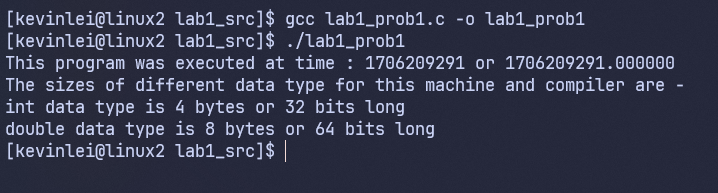
\includegraphics[width=0.75\textwidth]{./images/prob1partb.png}
    \caption{Compiling and running \lstinline!lab1_prob1.c!}
\end{figure}

\subsection{Part C}
The \lstinline!timeval! struct contains the \lstinline!tv_sec! variable, which is a numeric value like int or double.

\newpage
\section{Problem 2}

\subsection{Part A}
\begin{figure}[H]
    \centering
    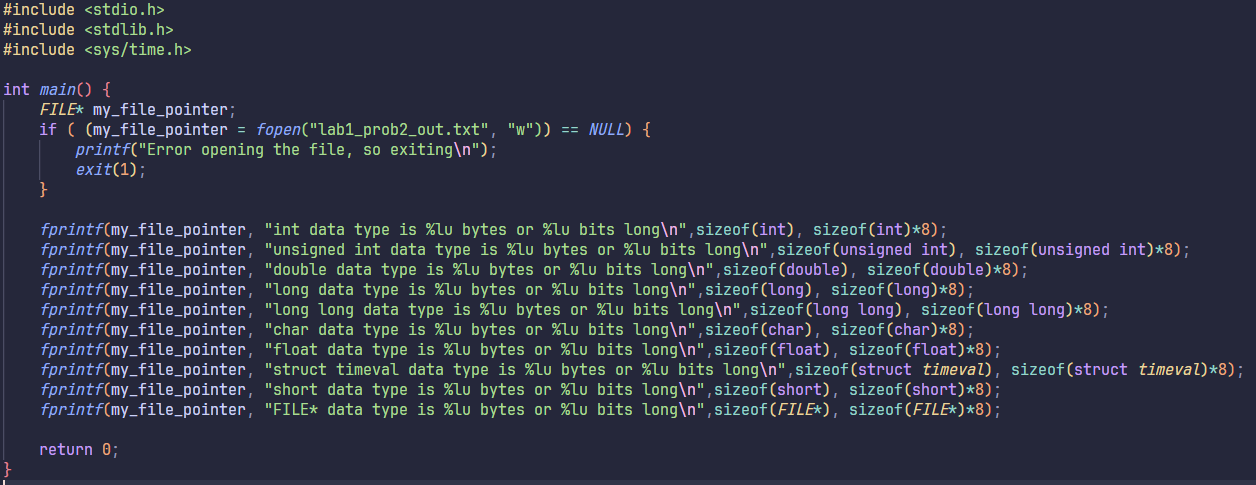
\includegraphics[width=1\textwidth]{./images/prob2parta1.png}
    \caption{Source code for \lstinline!lab1_prob2.c!}
\end{figure}

\begin{figure}[H]
    \centering
    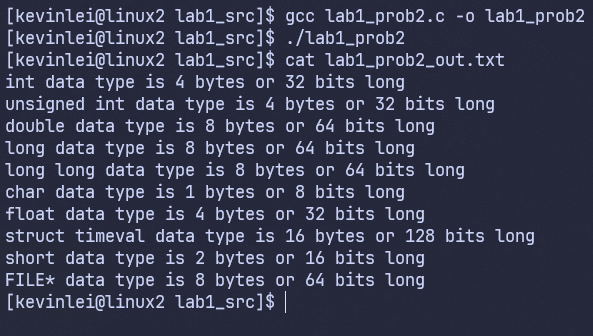
\includegraphics[width=0.75\textwidth]{./images/prob2parta2.png}
    \caption{Compiling and running \lstinline!lab1_prob2.c!, including the output.}
\end{figure}

\newpage
\subsection{Part B}
The structs \lstinline!employee1! and \lstinline!employee2! have the same bit and byte sizes of  448 bits and 56 bytes respectively.
In theory, the structs should use different amounts of memory.
Although they both have an int field, the \lstinline!employee2! struct has an array of characters of maximum length 52, 
while the \lstinline!employee1! struct has an array of characters of maximum length 50.
The code and output are shown below.

\begin{figure}[H]
    \centering
    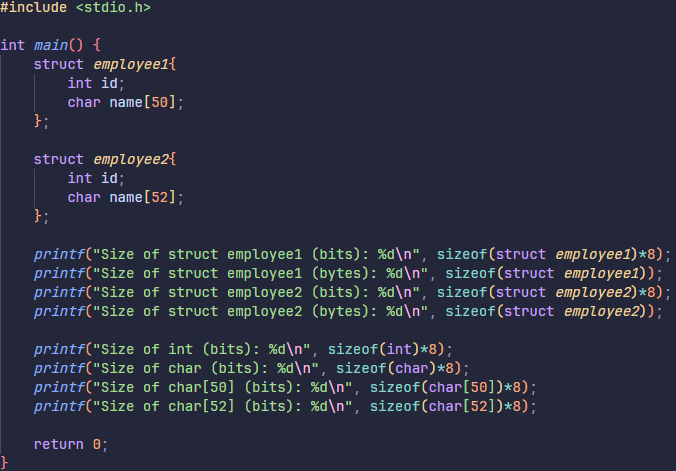
\includegraphics[width=0.75\textwidth]{./images/prob2partb1.png}
    \caption{Source code for \lstinline!lab1_prob2b.c!}
\end{figure}

\begin{figure}[H]
    \centering
    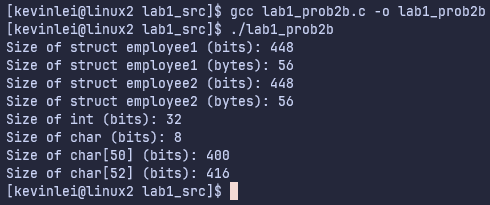
\includegraphics[width=0.75\textwidth]{./images/prob2partb2.png}
    \caption{Compiling and running \lstinline!lab1_prob2b.c!, including the output.}
\end{figure}

As we can see in the screenshots, the structs have the same bit and byte sizes,
However, \lstinline!char name[50]! and \lstinline!char name[52]! have difference bit sizes, 400 and 416 respectively.
Adding 416 to 32 bits for the int field gives us 448 bits, which is the same as the bit size of the struct.
This makes sense for the \lstinline!employee2! struct, but not for the \lstinline!employee1! struct, since 400 + 32 = 432, not 448.
The reason for this is called memory alignment, which is where memory chunks are organized into multiples of certain sizes.
These sizes are typically the largest data type that can be handled by the processor.
In this case, since the largest data type is \lstinline!employee2! which uses 448 bits, the memory is aligned to 448 bits, and 448 bits are also allocated for \lstinline!employee1!.

\newpage
\section{Problem 3}

\subsection{Part A}
\textbf{Bell actuator truth table:}
\\
\begin{tabular} {c c c c c c c c | c}
    \hline
    DSBF & ER & DC & DLC & DOS & KIC & BP & CM & BELL \\
    \hline
    0 & 0 & 0 & X & X & X & X & X & 0 \\
    1 & 0 & 0 & X & X & X & X & X & 0 \\
    0 & 0 & 1 & X & X & X & X & X & 0 \\
    1 & 0 & 1 & X & X & X & X & X & 0 \\
    0 & 1 & 0 & X & X & X & X & X & 1 \\
    1 & 1 & 0 & X & X & X & X & X & 1 \\
    0 & 1 & 1 & X & X & X & X & X & 1 \\
    1 & 1 & 1 & X & X & X & X & X & 0 \\
\end{tabular}
\\

\noindent\textbf{Door Lock actuator truth table:}
\\
\begin{tabular} {c c c c c c c c | c}
    \hline
    DSBF & ER & DC & DLC & DOS & KIC & BP & CM & DLA \\
    \hline
    X & X & X & 1 & 0 & 0 & X & X & 1 \\
    X & X & X & 1 & 1 & 0 & X & X & 1 \\
    X & X & X & 1 & 0 & 1 & X & X & 0 \\
    X & X & X & 1 & 1 & 1 & X & X & 1 \\
    X & X & X & 0 & 0 & 0 & X & X & 0 \\
    X & X & X & 0 & 1 & 0 & X & X & 0 \\
    X & X & X & 0 & 0 & 1 & X & X & 0 \\
    X & X & X & 0 & 1 & 1 & X & X & 0 \\
\end{tabular}
\\

\noindent\textbf{Brake actuator truth table:}
\\
\begin{tabular} {c c c c c c c c | c}
    \hline
    DSBF & ER & DC & DLC & DOS & KIC & BP & CM & BA \\
    \hline
    X & X & X & X & X & X & 0 & 0 & 0 \\
    X & X & X & X & X & X & 1 & 0 & 0 \\
    X & X & X & X & X & X & 0 & 1 & 0 \\
    X & X & X & X & X & X & 1 & 1 & 1 \\
\end{tabular}
\\

\subsection{Part B}
The boolean expressions for the Bell actuator, Door Lock actuator, and Brake actuator are shown below.
\begin{align*}
    BELL &= ER * (DSBF' + DC') \\
    DLA &= DLC * (KIC' + DOS) \\
    BA &= BP * CM
\end{align*}

\subsection{Part C}
\begin{figure}[H]
    \centering
    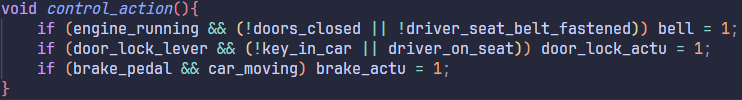
\includegraphics[width=0.75\textwidth]{./images/prob3partc.png}
    \caption{Source code for control system.}
\end{figure}

\subsection{Part D}
\begin{figure}[H]
    \centering
    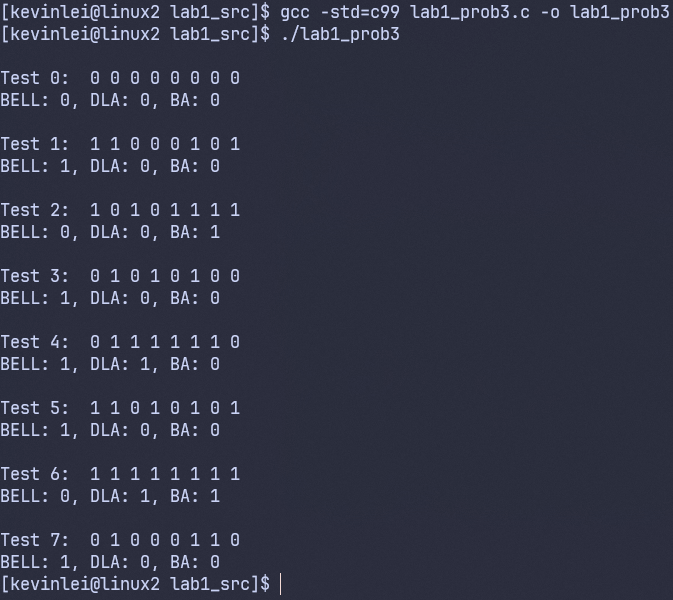
\includegraphics[width=0.75\textwidth]{./images/prob3partd.png}
    \caption{Compiling and running \lstinline!lab1_prob3.c!, including the output.}
\end{figure}

\section{Problem 4}



\section{Problem 5}

\end{document}
